\documentclass[border=4pt]{standalone}
% Shared style for every diagram. Colour-blind-safe palette (Okabe-Ito).
\usepackage[T1]{fontenc}
\usepackage{helvet}
\renewcommand{\familydefault}{\sfdefault}
\usepackage{tikz}
\usetikzlibrary{arrows.meta,positioning,fit,backgrounds,calc,shapes.geometric,decorations.pathreplacing}
\definecolor{cblue}{HTML}{0072B2}
\definecolor{corange}{HTML}{E69F00}
\definecolor{cgreen}{HTML}{009E73}
\definecolor{cred}{HTML}{D55E00}
\definecolor{cpurple}{HTML}{CC79A7}
\definecolor{cgrey}{HTML}{6B7280}
\definecolor{csky}{HTML}{56B4E9}
\tikzset{
  >={Stealth[length=2.2mm]},
  box/.style={draw, rounded corners=3pt, align=center, minimum height=11mm, minimum width=22mm, font=\small, line width=0.7pt},
  real/.style={box, draw=cblue, fill=cblue!8},
  sim/.style={box, draw=corange, fill=corange!12},
  future/.style={box, draw=cgrey, dashed, fill=white},
  flow/.style={->, line width=0.8pt, draw=black!75},
  dflow/.style={->, line width=0.8pt, dashed, draw=cgrey},
  lbl/.style={font=\scriptsize, text=black!70},
  group/.style={draw=black!25, rounded corners=6pt, inner sep=6pt},
}

\begin{document}
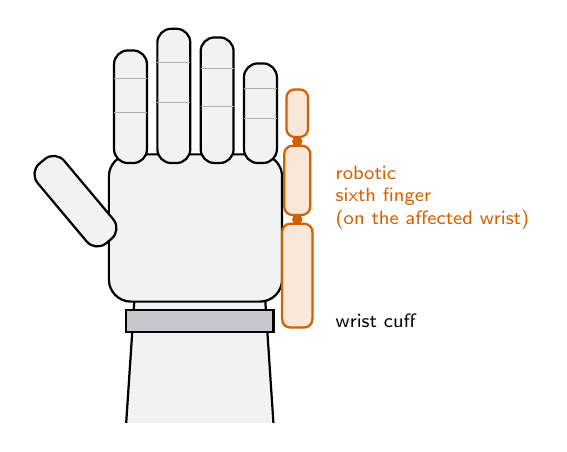
\begin{tikzpicture}[scale=0.55, line width=0.8pt]
  % forearm and palm
  \draw[fill=black!5] (-1.6,-4) -- (-1.4,-1) -- (1.6,-1) -- (1.8,-4);
  \draw[fill=black!5, rounded corners=8pt] (-2,-1.2) rectangle (2,2.2);
  % fingers
  \foreach \x/\h in {-1.5/2.6, -0.5/3.1, 0.5/2.9, 1.5/2.3} {
    \draw[fill=black!5, rounded corners=5pt] (\x-0.38,2.0) rectangle (\x+0.38,2.0+\h);
    \draw[black!30, line width=0.4pt] (\x-0.38,2.0+\h*0.45) -- (\x+0.38,2.0+\h*0.45);
    \draw[black!30, line width=0.4pt] (\x-0.38,2.0+\h*0.75) -- (\x+0.38,2.0+\h*0.75);
  }
  % thumb
  \draw[fill=black!5, rounded corners=5pt, rotate around={40:(-2,0.2)}] (-2.4,0.2) rectangle (-1.6,2.6);
  % wrist cuff and robotic sixth finger on the ulnar side
  \draw[fill=cgrey!40] (-1.6,-1.9) rectangle (1.8,-1.4);
  \draw[draw=cred, fill=cred!15, rounded corners=3pt] (2.0,-1.8) rectangle (2.7,0.6);
  \draw[draw=cred, fill=cred!15, rounded corners=3pt] (2.05,0.8) rectangle (2.65,2.4);
  \draw[draw=cred, fill=cred!15, rounded corners=3pt] (2.1,2.6) rectangle (2.6,3.7);
  \foreach \y in {0.7,2.5} \fill[cred] (2.35,\y) circle (0.12);
  \node[font=\scriptsize, text=cred, anchor=west, align=left] at (3.0,1.2) {robotic\\sixth finger\\(on the affected wrist)};
  \node[font=\scriptsize, anchor=west, align=left] at (3.0,-1.65) {wrist cuff};
\end{tikzpicture}
\end{document}
